\documentclass[a4paper]{article}
\usepackage{cmap}
\usepackage[utf8]{inputenc}
\usepackage[T2A]{fontenc}
\usepackage[english,russian]{babel} 
\usepackage[left=15mm, top=15mm, right=15mm, bottom=42mm, nohead, nofoot]{geometry}
\usepackage{blindtext}  % рыба-текст
\usepackage{graphicx}  % изобржаения
\usepackage{float} % плавающие объекты
\usepackage{wrapfig}  % изобржаения
\usepackage{tikz} % графика
\usepackage{xcolor} % определение цветов
\usepackage{nicefrac} % красивые дроби
\usepackage{cancel} % сокращение
\usepackage{amsmath,amsfonts,amssymb} % математический пакет
\usepackage{hyperref}  % гиперссылки
\usepackage{fancybox,fancyhdr} % хедер и футер
\usepackage{listings} % код
\usepackage{accsupp}
\usepackage{caption}
\usepackage{graphicx}
\captionsetup[figure]{name=Рисунок}
\pagestyle{fancy}
\fancyhf{}
\fancyhead[L]{Лабораторная работа №1}
\fancyhead[R]{\textit{Формы представления линейных динамических систем}}
\fancyfoot[C]{\thepage}
\headsep=8mm
\footskip=20mm

\definecolor{urlcolor}{HTML}{3454D1}
\definecolor{linkcolor}{HTML}{3454D1}
\hypersetup{pdfstartview=FitH, linkcolor=linkcolor, urlcolor=urlcolor, colorlinks=true}

\definecolor{strings}{rgb}{0,0.6,0}
\definecolor{comments}{rgb}{0,0.3,0}
\definecolor{numbers}{rgb}{0.5,0.5,0.5}
\definecolor{keywords}{rgb}{0.09,0.61,0.95}
\definecolor{background}{rgb}{0.97,0.97,0.97}
\newcommand{\noncopynumber}[1]{%
    \BeginAccSupp{method=escape,ActualText={}}%
    #1%
    \EndAccSupp{}%
}
\lstdefinestyle{codestyle}{
    backgroundcolor=\color{background},
    commentstyle=\color{comments},
    keywordstyle=\color{keywords},
    stringstyle=\color{strings},
    numberstyle=\tiny\color{numbers}\noncopynumber,
    basicstyle=\ttfamily\footnotesize,
    breakatwhitespace=false,
    breaklines=true,
    captionpos=b,
    inputencoding=utf8,
    keepspaces=true,
    numbers=left,
    numbersep=5pt,
    showspaces=false,
    showstringspaces=false,
    showtabs=false,
    tabsize=2,
    extendedchars=true,
    literate=
    {а}{{\cyra}}1
    {б}{{\cyrb}}1
    {в}{{\cyrv}}1
    {г}{{\cyrg}}1
    {д}{{\cyrd}}1
    {е}{{\cyre}}1
    {ж}{{\cyrzh}}1
    {з}{{\cyrz}}1
    {и}{{\cyri}}1
    {й}{{\cyrishrt}}1
    {к}{{\cyrk}}1
    {л}{{\cyrl}}1
    {м}{{\cyrm}}1
    {н}{{\cyrn}}1
    {о}{{\cyro}}1
    {п}{{\cyrp}}1
    {р}{{\cyrr}}1
    {с}{{\cyrs}}1
    {т}{{\cyrt}}1
    {у}{{\cyru}}1
    {ф}{{\cyrf}}1
    {х}{{\cyrh}}1
    {ц}{{\cyrc}}1
    {ч}{{\cyrch}}1
    {ш}{{\cyrsh}}1
    {щ}{{\cyrshch}}1
    {ъ}{{\cyrhrdsn}}1
    {ы}{{\cyrery}}1
    {ь}{{\cyrsftsn}}1
    {э}{{\cyrerev}}1
    {ю}{{\cyryu}}1
    {я}{{\cyrya}}1
    {А}{{\CYRA}}1
    {Б}{{\CYRB}}1
    {В}{{\CYRV}}1
    {Г}{{\CYRG}}1
    {Д}{{\CYR96}}1
    {Е}{{\CYRE}}1
    {Ж}{{\CYRZH}}1
    {З}{{\CYRZ}}1
    {И}{{\CYRI}}1
    {Й}{{\CYRISHRT}}1
    {К}{{\CYRK}}1
    {Л}{{\CYRL}}1
    {М}{{\CYRM}}1
    {Н}{{\CYRN}}1
    {О}{{\CYRO}}1
    {П}{{\CYRP}}1
    {Р}{{\CYRR}}1
    {С}{{\CYRS}}1
    {Т}{{\CYRT}}1
    {У}{{\CYRU}}1
    {Ф}{{\CYRF}}1
    {Х}{{\CYRH}}1
    {Ц}{{\CYRC}}1
    {Ч}{{\CYRCH}}1
    {Ш}{{\CYRSH}}1
    {Щ}{{\CYRSHCH}}1
    {Ъ}{{\CYRHRDSN}}1
    {Ы}{{\CYRERY}}1
    {Ь}{{\CYRSFTSN}}1
    {Э}{{\CYREREV}}1
    {Ю}{{\CYRYU}}1
    {Я}{{\CYRYA}}1
}

\lstset{style=codestyle}

\addto\captionsrussian{
  \renewcommand{\contentsname}
    {\centering Содержание}
}


\newlength{\tempheight}
\newcommand{\Let}{
\mathbin{\text{\settoheight{\tempheight}{\mathstrut}\raisebox{0.4\pgflinewidth}{
\tikz[baseline=0.5ex,line cap=round,line join=round] \draw (0,0) --++ (0.3em,0) --++ (0,2.3ex) --++ (-0.3em,0);
}}}}
\newcommand*\squared[1]{\tikz[baseline=(char.base)]{
            \node[shape=rectangle,draw,inner sep=4pt] (char) {#1};}}
\newcommand*\msquared[1]{\tikz[baseline=(char.base)]{
            \node[shape=rectangle,draw,inner sep=4pt] (char) {$\displaystyle #1$};}}
\newcommand{\at}{\biggr\rvert}
\newcommand{\shiftright}[3]{\makebox[#2][r]{\makebox[#1][l]{#3}}}
\newcommand{\e}{\;\text{e}}
\let\oldint\int
\def\int{\oldint\limits}
\DeclareRobustCommand{\divby}{%
  \mathrel{\vbox{\baselineskip.65ex\lineskiplimit0pt\hbox{.}\hbox{.}\hbox{.}}}%
}

\newcommand\NB{\textbf{N\kern-0.32em\textcolor{red}{B}}}

\begin{document}

\begin{titlepage}
    \begin{center}
        Федеральное государственное автономное образовательное \\ учреждение высшего образования \\[6pt]
        САНКТ-ПЕТЕРБУРГСКИЙ НАЦИОНАЛЬНЫЙ \\ ИССЛЕДОВАТЕЛЬСКИЙ УНИВЕРСИТЕТ ИТМО \\[16pt]
        Факультет систем управления и робототехники \\[26em]
        Лабораторная работа №1\\[0.5em]
        \textbf{ФОРМЫ ПРЕДСТАВЛЕНИЯ ЛИНЕЙНЫХ ДИНАМИЧЕСКИХ СИСТЕМ}
    \end{center}\,\\[10em]
    \begin{flushright}
        Студент: Заводин Е.Ю.\\
        Лин САУ R23 бак 1.1.1 \\[0.5em]
        Преподаватели: Перегудин А.А.\\
        Пашенко А.В.
    \end{flushright}\,\\[6em]
    \begin{center}
        {\small Санкт-Петербург \\ 2025}
    \end{center}
\end{titlepage}
\setcounter{page}{2}
\tableofcontents\newpage

\section{Одноканальная система в форме вход-выход}\

Согласно указанному в таблице с результатами успеваемости варианту 6, мои коэффициенты для выполнения этого задания следующие:\

$$
a_2 = 10, a_1 = 31, a_0 = 30, b_2 = 36, b_1 = 21, b_0 = 21.
$$\

Соответственно, модель в форме дифференциального уравнения выглядит следующим образом:\

$$
\dddot{y}+10\,\ddot{y}+31\,\dot{y} + 30\,y = 36\,\ddot{u} + 21\,\dot{u} + 21\,u.
$$\

Введём оператор дифференцирования $p = \frac{d}{dt}$, перепишем систему с его использованием:\

$$
p^3[y]+10\,p^2[y]+31\,p[y] + 30\,y = 36\,p^2[u] + 21\,p[u] + 21\,u.
$$\

Теперь перенесём все члены полинома, кроме $p^3[y]$, в правую сторону уравнения относительно знака ``равно'', и, благодаря ``Операционному исчислению'' Оливера Хевисайда без малейших колебаний поделим всё уравнение на член, оставшийся в левой его части, получим

$$
y = \frac{1}{p^3}(21u-30y)+\frac{1}{p^2}(21u-31y)+\frac{1}{p}(36u-10y).
$$

Полученное ДУ легко представимо в виде структурной схемы.\

\begin{figure}[H]
    \centering
    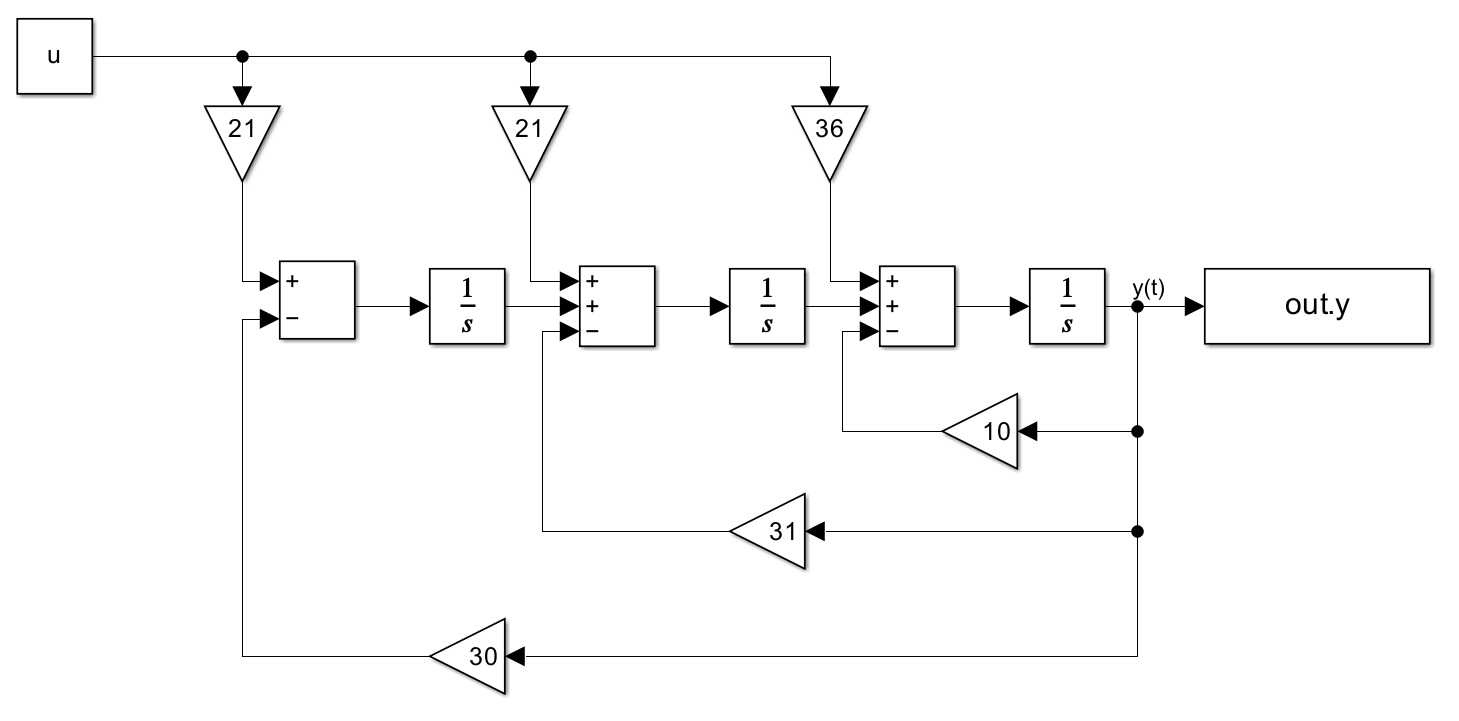
\includegraphics[width=0.75\linewidth]{ex1/structure_scheme.png}
    \caption{Структурная схема одноканальной системы В-В}
\end{figure}

Для анализа этой системы можно выполнить её моделирование при входном воздействии вида $u(t) = 1$ и нулевых начальных условиях $\ddot{y}(0), \dot{y}(0), y(0)$. Сделаю это, запустив соответствующий скрипт в MATLAB, вот полученные результаты:

\begin{figure}[H]
    \begin{minipage}{0.5\textwidth}
        \centering 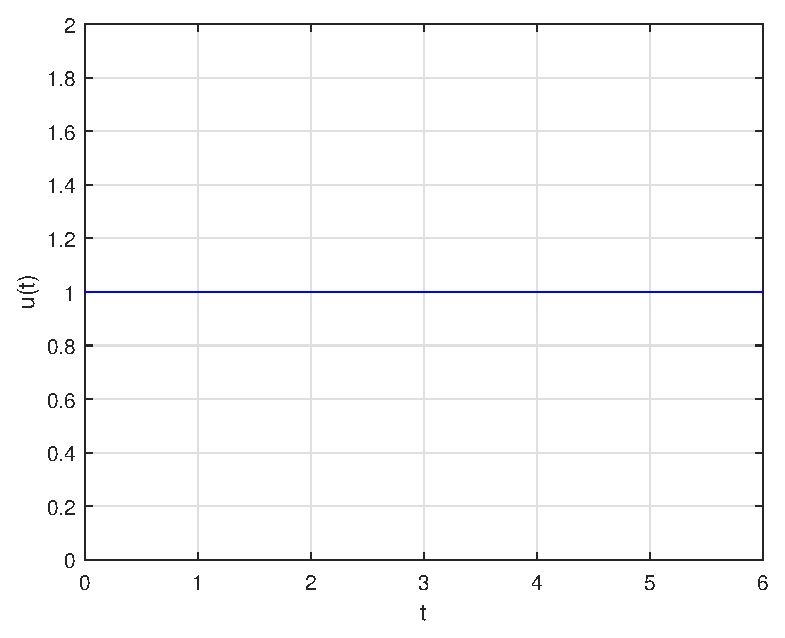
\includegraphics[width=\textwidth]{ex1/u.eps}
        \caption{График $u(t)$}
    \end{minipage}\hfill
    \begin{minipage}{0.5\textwidth}
        \centering 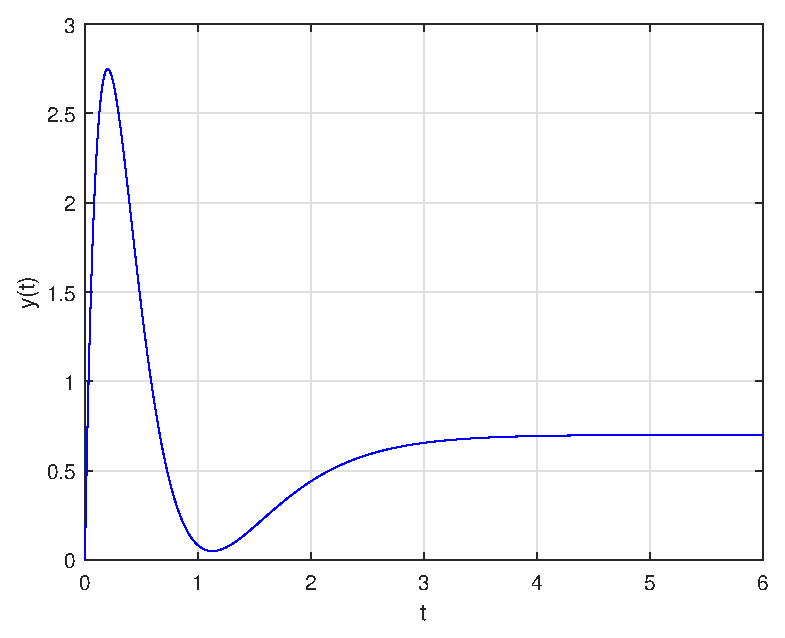
\includegraphics[width=\textwidth]{ex1/y.eps}
        \caption{График $y(t)$}
    \end{minipage}\\[1em]
\end{figure}\noindent\

\section{Переход от формы вход-выход к форме вход-состояние-выход}\

\subsection{Математические модели системы}

Для построения математических моделей в форме вход-состояние-выход для начала найду передаточную функцию системы. Для этого в исходном дифференциальном уравнении введу дифференциальный оператор, вынесу $y$ и $u$ за скобки и поделю на линейный дифференциальный оператор, стоящий перед $y$: 

$$
p^3[y]+10\,p^2[y]+31\,p[y] + 30\,y = 36\,p^2[u] + 21\,p[u] + 21\,u \Leftrightarrow
$$\

$$
\Leftrightarrow (p^3+10\,p^2+31\,p + 30)[y] = (36\,p^2 + 21\,p + 21)[u]\Leftrightarrow y = \frac{36\,p^2 + 21\,p + 21}{p^3+10\,p^2+31\,p + 30} [u] = W(p)[u]
$$\

Передаточная функция в виде дифференциально-интегрального оператора найдена. Это уже позволяет построить 2 из 3 требуемых канонических форм мат. модели вход-состояние-выход.\ 

\subsubsection{Общий вид канонических форм}\ 

В общем виде мат.модели в канонической управляемой и наблюдаемой формах для передаточной функции вида $W(p) = \frac{b_2p^2 + b_1p + b_0}{p^3+a_2p^2+a_1p+a_0}$ схожи.\ 

Каноническая управляемая:

$$
\begin{bmatrix}
    \dot{x_1} \\
    \dot{x_2} \\
    \dot{x_3}
\end{bmatrix} = \begin{bmatrix}
    0 & 1 & 0 \\ 
    0 & 0 & 1 \\
    -a_0 & -a_1 & -a_2
\end{bmatrix}\begin{bmatrix}
    x_1 \\
    x_2 \\
    x_3
\end{bmatrix} + \begin{bmatrix}
    0 \\ 
    0 \\ 
    1
\end{bmatrix}u
$$\

$$
y = \begin{bmatrix}
    b_0 & b_1 & b_2
\end{bmatrix}\begin{bmatrix}
    x_1 \\
    x_2 \\
    x_3
\end{bmatrix}
$$\

Каноническая наблюдаемая:

$$
\begin{bmatrix}
    \dot{x_1} \\
    \dot{x_2} \\
    \dot{x_3}
\end{bmatrix} = \begin{bmatrix}
    0 & 0 & -a_0 \\ 
    1 & 0 & -a_1 \\
    0 & 1 & -a_2
\end{bmatrix}\begin{bmatrix}
    x_1 \\
    x_2 \\
    x_3
\end{bmatrix} + \begin{bmatrix}
    b_0 \\ 
    b_1 \\ 
    b_2
\end{bmatrix}u
$$\

$$
y = \begin{bmatrix}
    0 & 0 & 1
\end{bmatrix}\begin{bmatrix}
    x_1 \\
    x_2 \\
    x_3
\end{bmatrix}
$$\

Общий вид канонической диагональной несколько отличается структурно от предыдущих. Для передаточной функции с динамическим порядком 3 и относительным динамическим 1 он выглядит следующим образом:

$$
\begin{bmatrix}
    \dot{x_1} \\
    \dot{x_2} \\
    \dot{x_3}
\end{bmatrix} = \begin{bmatrix}
    \lambda_1 & 0 & 0 \\ 
    0 & \lambda_2 & 0 \\
    0 & 0 & \lambda_3
\end{bmatrix}\begin{bmatrix}
    x_1 \\
    x_2 \\
    x_3
\end{bmatrix} + \begin{bmatrix}
    \beta_1 \\ 
    \beta_2 \\ 
    \beta_3
\end{bmatrix}u
$$\

$$
y = \begin{bmatrix}
    \gamma_1 & \gamma_2 & \gamma_3
\end{bmatrix}\begin{bmatrix}
    x_1 \\
    x_2 \\
    x_3
\end{bmatrix},
$$
где $\lambda_n$ -- корни знаменателя передаточной функции, $\beta_n\gamma_n = c_n$, где $c_n$ -- коэффициенты в разложении передаточной функции на простейшие дроби.

\subsubsection{Математические модели системы в управляемой и наблюдаемой формах}\ 

Для получения требуемой управляемой формы системы просто подставлю коэффициенты полиномов числителя и знаменателя передаточной функции в общий вид соответствующей модели:

$$
\begin{bmatrix}
    \dot{x_1} \\
    \dot{x_2} \\
    \dot{x_3}
\end{bmatrix} = \begin{bmatrix}
    0 & 1 & 0 \\ 
    0 & 0 & 1 \\
    -30 & -31 & -10
\end{bmatrix}\begin{bmatrix}
    x_1 \\
    x_2 \\
    x_3
\end{bmatrix} + \begin{bmatrix}
    0 \\ 
    0 \\ 
    1
\end{bmatrix}u
$$

$$
y = \begin{bmatrix}
    21 & 21 & 36
\end{bmatrix}\begin{bmatrix}
    x_1 \\
    x_2 \\
    x_3
\end{bmatrix}
$$\

Теперь на очереди каноническая наблюдаемая форма. Снова подставлю коэффициенты передаточной функции:

$$
\begin{bmatrix}
    \dot{x_1} \\
    \dot{x_2} \\
    \dot{x_3}
\end{bmatrix} = \begin{bmatrix}
    0 & 0 & -30 \\ 
    1 & 0 & -31 \\
    0 & 1 & -10
\end{bmatrix}\begin{bmatrix}
    x_1 \\
    x_2 \\
    x_3
\end{bmatrix} + \begin{bmatrix}
    21 \\ 
    21 \\ 
    36
\end{bmatrix}u
$$\

$$
y = \begin{bmatrix}
    0 & 0 & 1
\end{bmatrix}\begin{bmatrix}
    x_1 \\
    x_2 \\
    x_3
\end{bmatrix}
$$\

Для составления мат. модели в канонической диагональной форме требуется разложить передаточную функцию на простые дроби (можем воспринимать дифференциально-интегральный оператор как функцию от $p$ благодаря трудам Оливера-Хевисайда). Для этого сперва найду корни знаменателя. Первый из них, $\lambda_1 = -2$, я подобрал подстановкой, остальные -- делением полиномов ``уголком'', в результате чего получил $\lambda_2 = -3, \lambda_3 = -5$. Тогда можно записать передаточную функцию следующим образом:

$$
W(p) = \frac{36\,p^2 + 21\,p + 21}{p^3+10\,p^2+31\,p + 30} = \frac{c_1}{p+2} + \frac{c_2}{p+3} + \frac{c_3}{p+5}
$$\ 

Коэффициенты $c_1, c_2, c_3$ могут быть найдены по методу неопределенных коэффициентов. Для начала приведу дроби в правой части к общему знаменателю:

$$
\frac{c_1}{p+2} + \frac{c_2}{p+3} + \frac{c_3}{p+5} = \frac{c_1(p+3)(p+5) + c_2(p+2)(p+5) + c_3(p+2)(p+3)}{(p+2)(p+3)(p+5)}.
$$\ 

Теперь приравняю изначальную передаточную функцию к тому, что получил, и избавлюсь от знаменателя:

$$
W(p) = \frac{36\,p^2 + 21\,p + 21}{p^3+10\,p^2+31\,p + 30} = \frac{c_1(p+3)(p+5) + c_2(p+2)(p+5) + c_3(p+2)(p+3)}{(p+2)(p+3)(p+5)} \Leftrightarrow
$$
$$
\Leftrightarrow 36\,p^2 + 21\,p + 21 = c_1(p+3)(p+5) + c_2(p+2)(p+5) + c_3(p+2)(p+3) \Leftrightarrow
$$
$$
\Leftrightarrow 36\,p^2 + 21\,p + 21 = c_1(p^2+8p+15) + c_2(p^2+7p+10) + c_3(p^2+5p+6)\Leftrightarrow
$$
$$
\Leftrightarrow 36\,p^2 + 21\,p + 21 = p^2(c_1+c_2+c_3) + p^1(8c_1+7c_2+5c_3)+p^0(15c_1+10c_2+6c_3).
$$\ 

Составлю систему, приравняв коэффициенты при одинаковых степенях $p$:

$$
\begin{cases}
36 = c_1 + c_2 + c_3 \\
21 = 8c_1 + 7c_2 + 5c_3 \\ 
21 = 15c_1 + 10c_2 + 6c_3
\end{cases}
$$\ 

Решив систему, получил $c_1 = 41, c_2 = -141, c_3 = 136$.\ 

Тогда $W(p) = \frac{41}{p+2}+\frac{-141}{p+3}+\frac{136}{p+5}$. Для нахождения диагональной формы требуется найти такие $\beta_n, \gamma_n$, что $c_n = \beta_n \gamma_n$. Пусть $\beta_1 = 41, \beta_2 = 141, \beta_3 = 68$, тогда $\gamma_1 = 1, \gamma_2 = -1, \gamma_3 = 2$.

Зная общий вид канонической диагональной формы, подставим найденные значения, получим мат. модель вход-состояние-выход в канонической диагональной форме:

$$
\begin{bmatrix}
    \dot{x_1} \\
    \dot{x_2} \\
    \dot{x_3}
\end{bmatrix} = \begin{bmatrix}
    -2 & 0 & 0 \\ 
    0 & -3 & 0 \\
    0 & 0 & -5
\end{bmatrix}\begin{bmatrix}
    x_1 \\
    x_2 \\
    x_3
\end{bmatrix} + \begin{bmatrix}
    41 \\ 
    141 \\ 
    68
\end{bmatrix}u
$$\

$$
y = \begin{bmatrix}
    1 & -1 & 2
\end{bmatrix}\begin{bmatrix}
    x_1 \\
    x_2 \\
    x_3
\end{bmatrix}
$$\

\subsection{Структурные схемы для представлений В-С-В и их моделирование}\

Структурные схемы строил при помощи $Simulink$ на основании уже полученных моделей.\ 

Структурная схема модели в канонической наблюдаемой форме:

\begin{figure}[H]
    \centering
    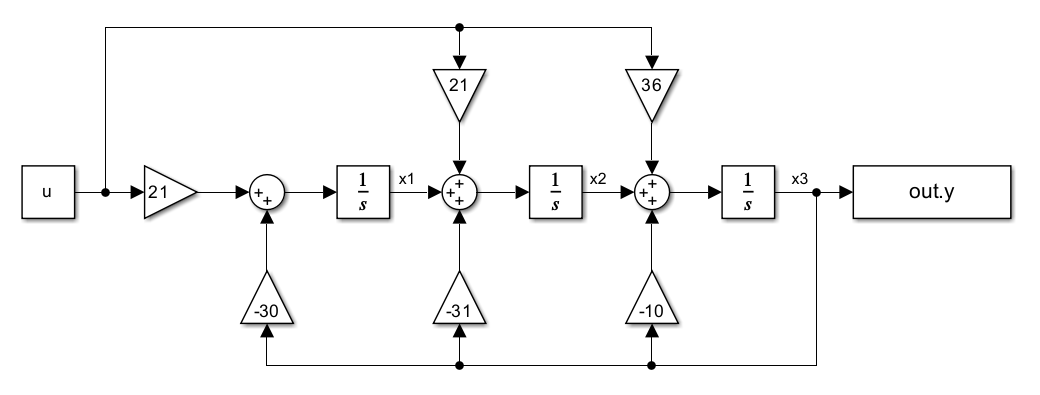
\includegraphics[width=0.75\linewidth]{ex2/scheme_observable.png}
    \caption{Структурная схема одноканальной системы В-С-В в наблюдаемой форме}
\end{figure}\

Структурная схема модели в канонической управляемой форме:

\begin{figure}[H]
    \centering
    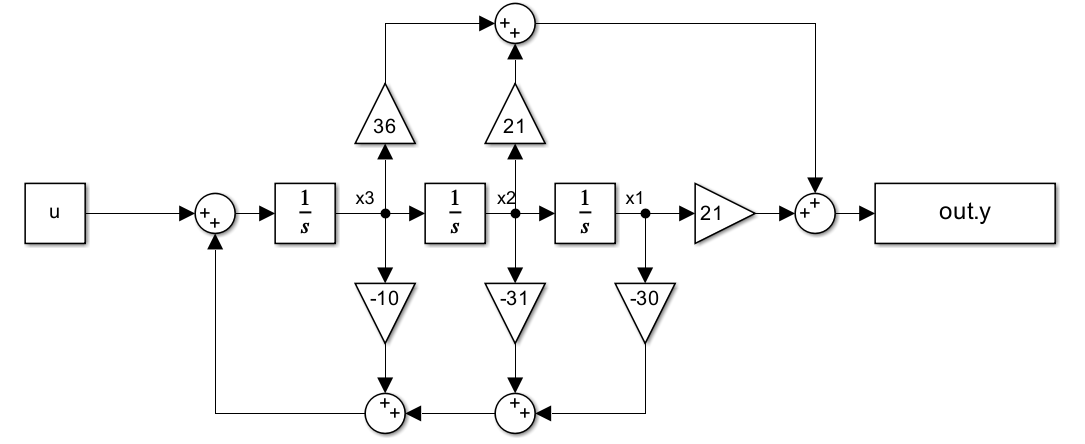
\includegraphics[width=0.75\linewidth]{ex2/scheme_controlable.png}
    \caption{Структурная схема одноканальной системы В-С-В в управляемой форме}
\end{figure}\

Структурная схема модели в канонической диагональной форме:

\begin{figure}[H]
    \centering
    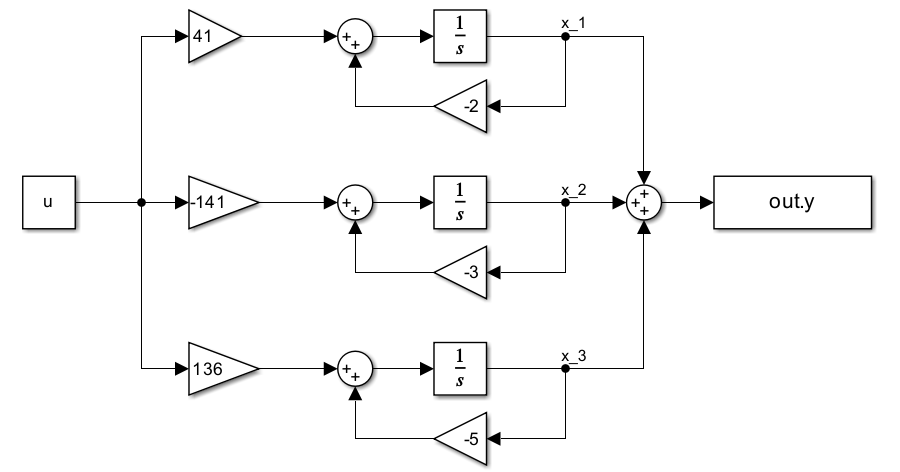
\includegraphics[width=0.75\linewidth]{ex2/scheme_diagonal.png}
    \caption{Структурная схема одноканальной системы В-С-В в диагональной форме}
\end{figure}\

Задал входное воздействие $u(t) = 1$, смоделировал передаточную функцию и полученные формы В-С-В:

\begin{figure}
    \centering
    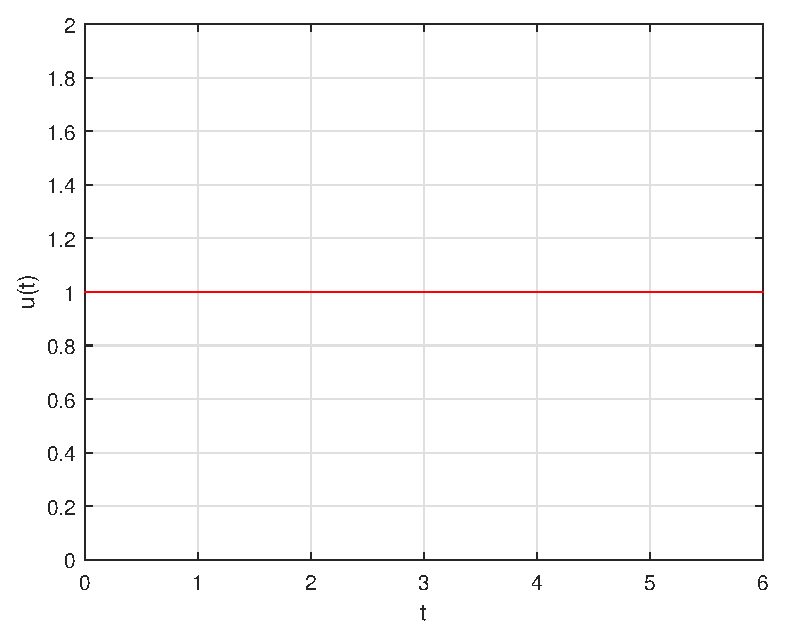
\includegraphics[width=0.75\linewidth]{ex2/u.eps}
    \caption{График $u(t)$}
\end{figure}

\begin{figure}
    \centering
    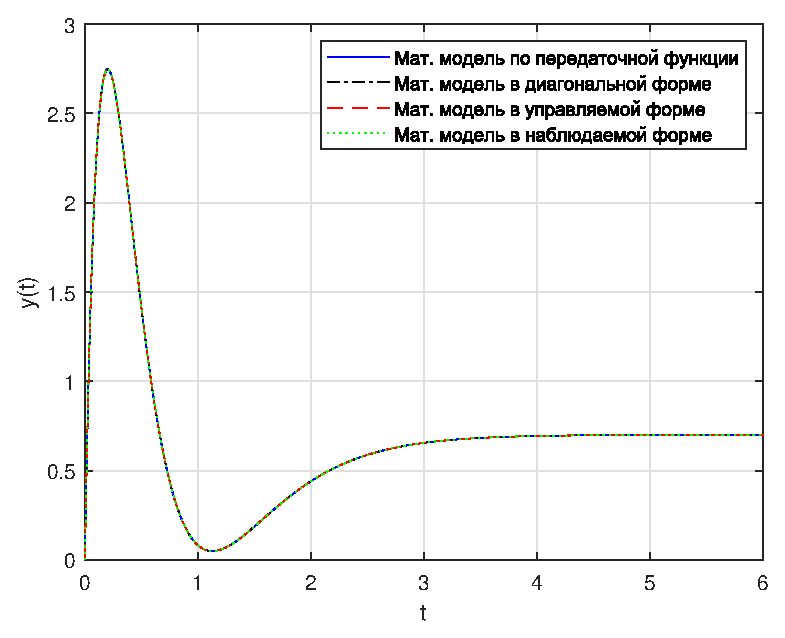
\includegraphics[width=0.75\linewidth]{ex2/y.eps}
    \caption{Графики $y(t)$}
\end{figure}

\subsection{Выводы}\

На графиках выходного сигнала можно заметить, что выходы от каждой из форм полностью идентичны, что говорит о том, что добавление в систему промежуточных состояний не меняет результата. Также графики выходных сигналов совпадают с графиком моделирования передаточной функции, из чего можно сделать вывод о том, что структурные схемы составлены верно.

\section{Многоканальная система в форме вход-выход}\

Рассмотрим систему вида\ 

$$
A(p)y(t) = B(p)u(t),
$$\ 

Для моего варианта:

$$
A(p) = \begin{bmatrix}
    p + 19 & p+3 \\ 
    p + 6 & p + 2
\end{bmatrix}, B(p) = \begin{bmatrix}
    7 & 7 \\
    5 & 6
\end{bmatrix}
$$\ 

Передаточную матрицу найду из соотношения $W(p) = A(p)^{-1}B(p)$, по аналогии с передаточной функцией в одноканальной системе.

$$
A(p)^{-1} = \frac{1}{det\,A(p)},adj(A(p)) =\frac{1}{det\,A(p)}A(p)_{ij}^T, \Rightarrow W(p) = \frac{1}{det\,A}A(p)_{ij}^T B(p)
$$
$$
detA(p) = (p+19)(p+2) - (p+3)(p+6) = p^2+19p+2p+38-p^2-3p-6p-18 = 12p+20
$$
$$
A(p)_{ij}^T=\begin{bmatrix}
    p+2 & -p-3 \\
    -p-6 & p+19
\end{bmatrix}
$$
значит,
$$
W(p) = \frac{1}{12p+20}\begin{bmatrix}
    p+2 & -p-3 \\
    -p-6 & p+19
\end{bmatrix}\begin{bmatrix}
    7 & 7 \\ 
    5 & 6
\end{bmatrix}= \frac{1}{12p+20}\begin{bmatrix}
    2p-1 & p-4 \\
    -2p+53 & -p+72
\end{bmatrix}
$$

По данной передаточной матрице была построена структурная схема системы:

\begin{figure}[H]
    \centering
    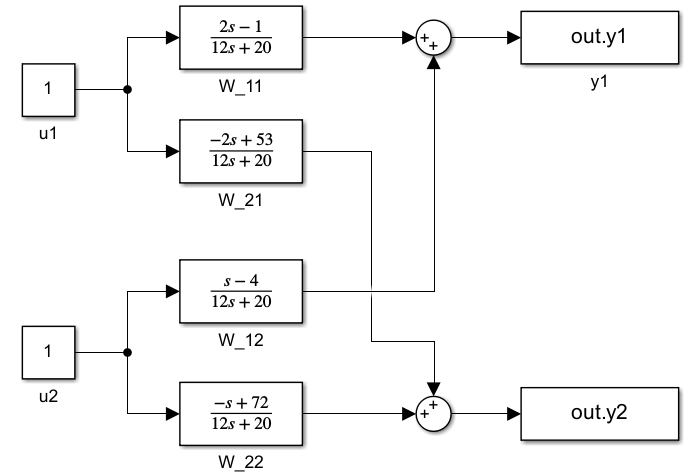
\includegraphics[width=0.65\linewidth]{ex3/scheme.png}
    \caption{Структурная схема многоканальной системы В-В}
\end{figure}

Схема была запущена с входными воздействиями $u_1 = 1(t)$ и $u_2 = sin(t)$ при нулевых начальных условиях:

\begin{figure}[H]
    \begin{minipage}{0.5\textwidth}
        \centering 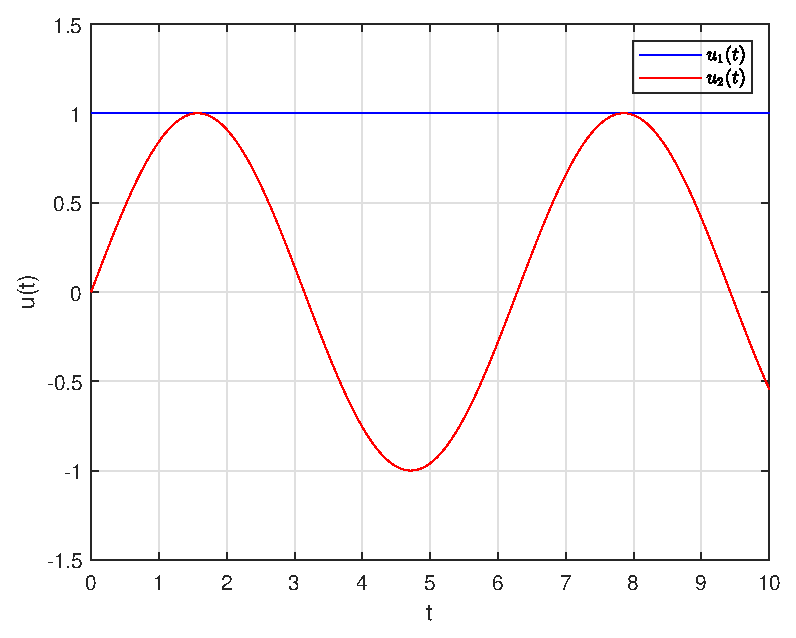
\includegraphics[width=\textwidth]{ex3/u.eps}
        \caption{График $u(t)$}
    \end{minipage}\hfill
    \begin{minipage}{0.5\textwidth}
        \centering 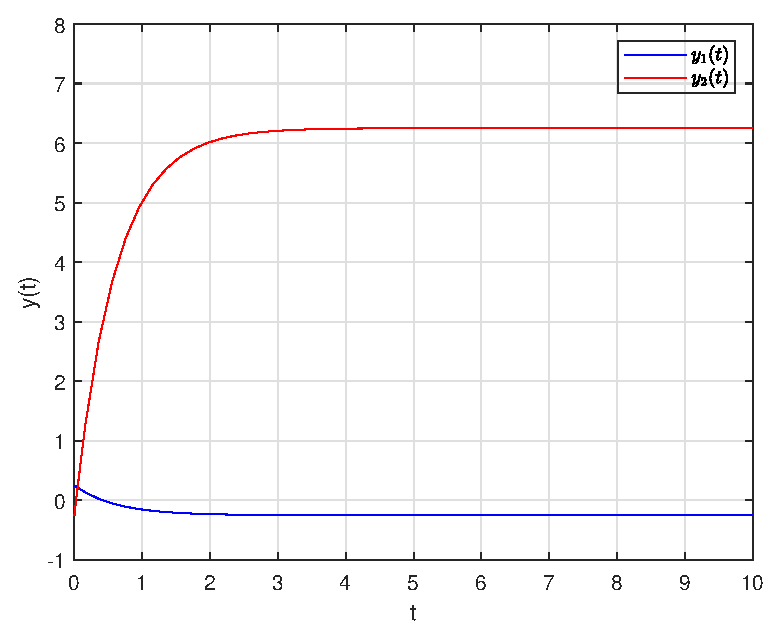
\includegraphics[width=\textwidth]{ex3/y.eps}
        \caption{Графики $y(t)$}
    \end{minipage}\\[1em]
\end{figure}\noindent\

\section{Многоканальная система в форме вход-состояние-выход}\

Общий вид используемой в задании многоканальной системы $Strictly\, Proper$ в форме В-С-В следующий:

$$
\begin{cases}
    \dot{x}=Ax+Bu \\
    y = Cx
\end{cases}
$$\ 

В качестве $A, B, C$ в соответствии с 6 вариантом были взяты следующие матрицы:

$$
A = \begin{bmatrix}
    0 & -9 \\ 
    1 & -6
\end{bmatrix}, B = \begin{bmatrix}
    1 & 4 \\
    3 & 5
\end{bmatrix}, C = \begin{bmatrix}
    2 & 7 \\ 
    4 & 6
\end{bmatrix}
$$\ 

Структурная схема, составленная в соответствии с полученной системой:

\begin{figure}[H]
    \centering
    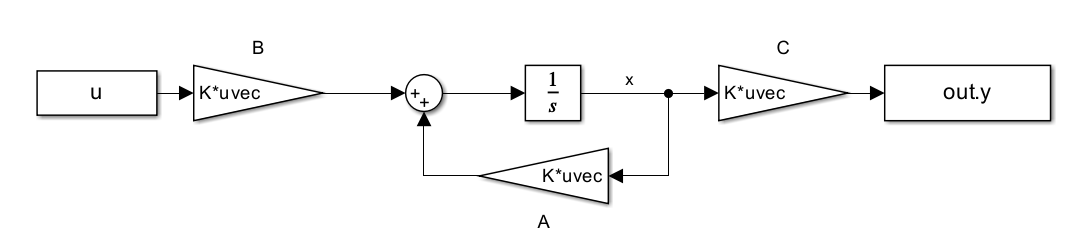
\includegraphics[width=0.65\linewidth]{ex4/scheme.png}
    \caption{Структурная схема многоканальной системы В-С-В}
\end{figure}\ 

Схема была смоделирована при начальных воздействиях $u_1(t) = 1$ и $u_2(t) = sin(t)$ и нулевом начальном значении вектора состояния:

\begin{figure}[H]
    \begin{minipage}{0.5\textwidth}
        \centering 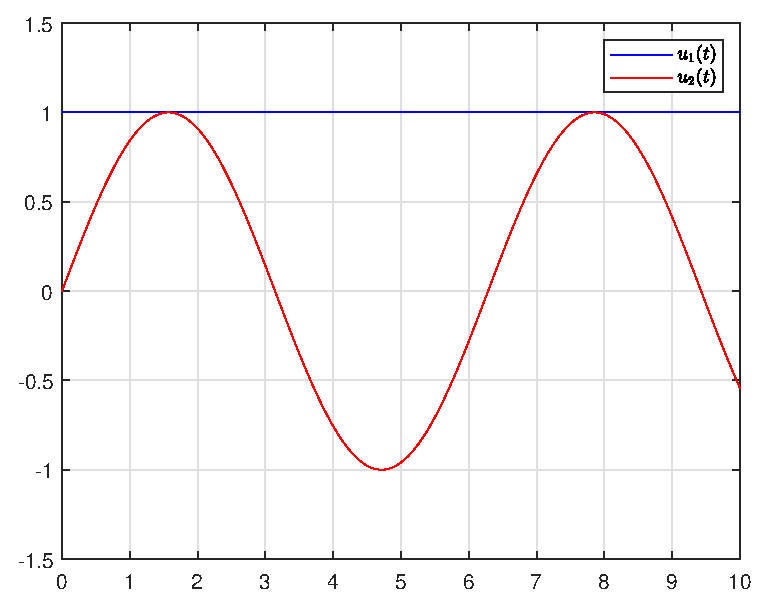
\includegraphics[width=\textwidth]{ex4/u.eps}
        \caption{График $u(t)$}
    \end{minipage}\hfill
    \begin{minipage}{0.5\textwidth}
        \centering 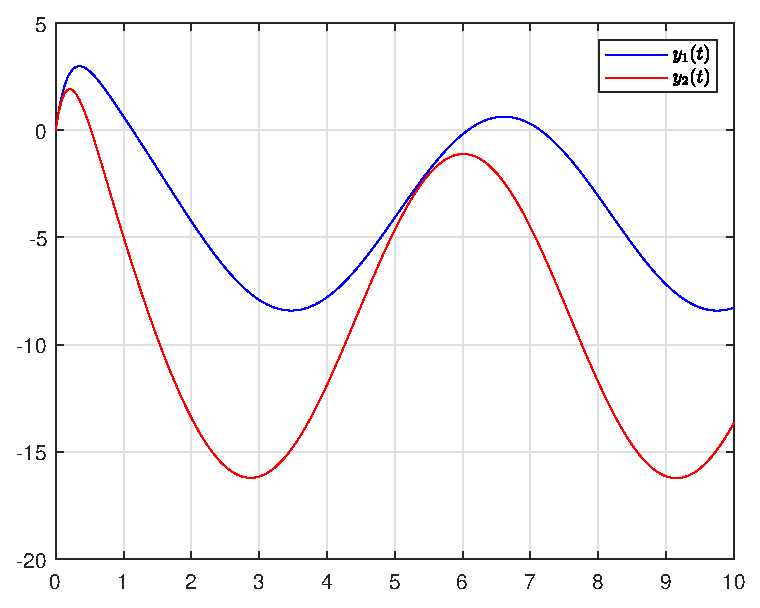
\includegraphics[width=\textwidth]{ex4/y.eps}
        \caption{Графики $y(t)$}
    \end{minipage}\\[1em]
    \caption{Графики многоканальной системы В-С-В}
\end{figure}\noindent\

По графикам выходного сигнала видно, что вход $u_2(t)$ действует на оба выхода, так как гармонические колебания появляются и на графике $y_1(t)$, и на $y_2(t)$. Амплитуда колебаний у $y_2(t)$ больше, поэтому можно предположить, что вход $u_2(t)$ оказывает на него большее влияние.

\section{Выводы}\

В процессе выполнения работы я научился более вдумчиво читать структурные схемы, а также создавать их, поработал с операторными передаточными функциями как с обычными функциями, а также познакомился с различными формами представления линейных систем, научился составлять их из передаточных функций (переходить от В-В к В-С-В).

\newpage

\section{Приложение А. Код для выполнения заданий}

\subsection*{Листинг 1. Код для выполнения задания 1}

\begin{lstlisting}[caption={Код для построения графиков для задания 1}, language=matlab]
u = ones(1000,1);

out = sim('model.slx','StopTime','6');
t = linspace(0, 999, 1000);
y = out.y;

u_t = figure;
plot(t, u, 'red'), grid on
xlim([0, 6]);
xlabel('t'), ylabel('u(t)')
title('График u(t)')

y_t = figure;
y.plot('black'), grid on
xlabel('t'), ylabel('y(t)')
title('График y(t)')
\end{lstlisting}


\subsection*{Листинг 2. Код для выполнения задания 2}

\begin{lstlisting}[caption={Код для построения графиков для задания 2}, language=matlab]
close all;
u = 1;

out = sim('model2_diagonal.slx','StopTime','6');
t = linspace(0, 6, 1000);
y_diagonal = out.y;

u_t = figure;
u1 = ones(size(t));
plot(t, u1, 'red'); grid on
xlim([0, 6]);
xlabel('t'), ylabel('u(t)')
title('График u(t)')

num = [36 21 21];
den = [1 10 31 30];
sys = tf(num, den);
y = lsim(sys, u1, t);
y_t = figure;
plot(t, y); grid on
xlabel('t'), ylabel('y(t)')
hold on;

y_diagonal.plot('black')
title('Графики y(t)')
hold on;

out = sim('model2_controlable.slx','StopTime','6');
y_controlable = out.y;
y_controlable.plot('--red')
hold on;

xlim([0, 6]);
out = sim('model2_observable.slx','StopTime','6');
y_observable = out.y;
y_observable.plot(':green')
grid on;
legend('Мат. модель по передаточной функции', 'Мат. модель в диагональной форме', 'Мат. модель в управляемой форме', 'Мат. модель в наблюдаемой форме')
\end{lstlisting}


\subsection*{Листинг 3. Код для выполнения задания 3}

\begin{lstlisting}[caption={Код для построения графиков для задания 3}, language=matlab]
close all;

t = (0:0.01:10);
u1 = ones(size(t));
u2 = sin(t);
out = sim('model3');

figure;
out.y1.plot('black')
title('Графики y(t)')
xlabel('t'); ylabel('y(t)')
hold on;

out.y2.plot('red')
grid on;
legend('$y_1(t)$', '$y_2(t)$', 'Interpreter', 'latex')

figure;
plot(t, u1, 'black')
hold on;
plot(t, u2, 'red')
xlabel('t'); ylabel('u(t)')
grid on
title('Графики u(t)')
ylim([-1.5, 1.5])
legend('$u_1(t)$', '$u_2(t)$', 'Interpreter', 'latex', BackgroundAlpha=.2)
\end{lstlisting}


\subsection*{Листинг 4. Код для выполнения задания 4}

\begin{lstlisting}[caption={Код для построения графиков для задания 4}, language=matlab]
close all;
t = (0:0.001:10)';
u = [t, ones(size(t)), sin(t)];

out = sim('model4');
plot(out.y.Time, out.y.Data(:, 1))
hold on;
plot(out.y.Time, out.y.Data(:, 2))
grid on;
legend('$y_1(t)$', '$y_2(t)$', 'Interpreter', 'latex')

figure
plot(t, u(:, 2))
hold on;
plot(t, u(:, 3))
grid on;
ylim([-1.5, 1.5])
legend('$u_1(t)$', '$u_2(t)$', 'Interpreter', 'latex')
\end{lstlisting}

\end{document}
